\documentclass[11pt]{article}
%% Packages:

\usepackage{amsmath}
\usepackage[document]{ragged2e}
\usepackage{titlesec}
\usepackage{float}
\usepackage{graphicx}
\usepackage{caption}
\usepackage{subcaption}
\usepackage[dvipsnames]{xcolor}
\usepackage[T1]{fontenc}
\usepackage{helvet}
\usepackage[hidelinks]{hyperref}
\usepackage[margin=2cm]{geometry}
\usepackage{amssymb}
\usepackage{enumitem}
\usepackage{comment}
\usepackage{soul}

%% Personalized adjustements: 

% Math operator:
\DeclareMathOperator{\sech}{sech}

% VUB colors: 
\definecolor{orange}{RGB}{234, 82, 0} 
\definecolor{blue}{RGB}{26, 55, 101}

% Margins:
\addtolength{\skip\footins}{0.3 cm}
\renewcommand*\footnoterule{}

% Adjustement of section, subsection & subsubsection: 

\titleformat{\section}[block]
{\normalfont\Large\bfseries \fontfamily{phv}\selectfont \color{orange}}
{\thesection}{0.5cm}{}

\titleformat{\subsection}[block]
{\normalfont\large\bfseries \fontfamily{phv}\selectfont \color{blue}}
{\thesubsection}{0.5cm}{}

\titleformat{\subsubsection}[block]
{\normalfont\small\bfseries \fontfamily{phv}\selectfont \color{blue}}
{\thesubsubsection}{0.5cm}{}
\usepackage{setspace}
\usepackage{graphicx}
\usepackage{subcaption}
\usepackage{parskip}
\usepackage{indentfirst}
\graphicspath{{Images/}}
%\setlength{\parindent}{1.5em}
\usepackage{float}
\onehalfspacing

\begin{document}
	\justifying
	
	\begin{titlepage}
	\begin{center}
            \begin{figure}
                \centering
                
\includegraphics[scale=0.3]{Images/logo.png}
            \end{figure}
		\vspace*{\fill}
            \normalsize
            {\fontfamily{phv}\selectfont
            \textcolor{blue}{\textbf{ELEC-H401}}}\\
            \vspace{0.2cm}
		\Huge
            {\fontfamily{phv}\selectfont
            \textcolor{orange}{Design and Simulation of a DVB-C Transmission Chain}}\\
        \end{center}
	\begin{center}	
		\vspace{0.5cm}
            \Large
            {\fontfamily{phv}\selectfont
			\textcolor{blue}{\textbf{Hadislam Satouev\\
                                 	 Cédric Sipakam
             }}}\\
	\end{center}
        \vspace*{\fill}
        \begin{FlushRight}
            {\fontfamily{phv}\selectfont
            \textcolor{orange}{Professor}}\\
            {\fontfamily{phv}\selectfont
            \textcolor{blue}{François Horlin}}\\
            \vspace{0.6cm}
            {\fontfamily{phv}\selectfont
            \textcolor{orange}{Teaching Assistants}}\\
            {\fontfamily{phv}\selectfont
            \textcolor{blue}{
                ....\\
                 ....
            }}\\
            \vspace{0.6cm}
            {\fontfamily{phv}\selectfont
            \textcolor{orange}{Academic Year}}\\
            {\fontfamily{phv}\selectfont
            \textcolor{blue}{2024 - 2025}}\\
            \vspace{0.6cm}
            {\fontfamily{phv}\selectfont
            \textcolor{orange}{Faculty}}\\
            {\fontfamily{phv}\selectfont
            \textcolor{blue}{Electrical Engineering}}
        \end{FlushRight}



\end{titlepage}
	\tableofcontents
	\newpage
	\listoffigures
	
	\newpage
	\section*{Introduction}{\addcontentsline{toc}{section}{Introduction}}
	This project focuses on designing and simulating a Digital Video Broadcasting Cable transmission chain using Matlab.
	The main goal is to model and analyze the components of a typical modem. The first part of this project includes establishing an optimal communication chain over an ideal Additive White Gaussian Noise channel, mapping the signal into symbols, Nyquist filtering, and evaluating the performance of the system through Bit Error Rate simulations for Quadrature Amplitude Modulation signals. The second part revolves around the design and assessment of time and frequency synchronization algorithms. This encompasses evaluating the impact of synchronization errors such as carrier phase and frequency offset and sample time shift. The algorithms used for this purpose are the Gardner Algorithm for time recovery, and a differential cross-correlator for joint frame and frequency acquisition. Afterwards, their effectiveness is demonstrated \textcolor{red}{through convergence analysis and residual error evaluation (double check)}. \textcolor{red}{The study also explores phase interpolation techniques to mitigate remaining phase drifts. Finally, the project aims to validate the simulated chain through real-life experimentation on a Hybrid Fiber-Coax setup using Adalm-Pluto hardware, and to compare the simulated performance with experimental observations.}
	
	
	\section{Optimal Communication Chain over the Ideal Channel}
	\subsection{Communication Chain}
	\begin{figure}[H]
		\centering
		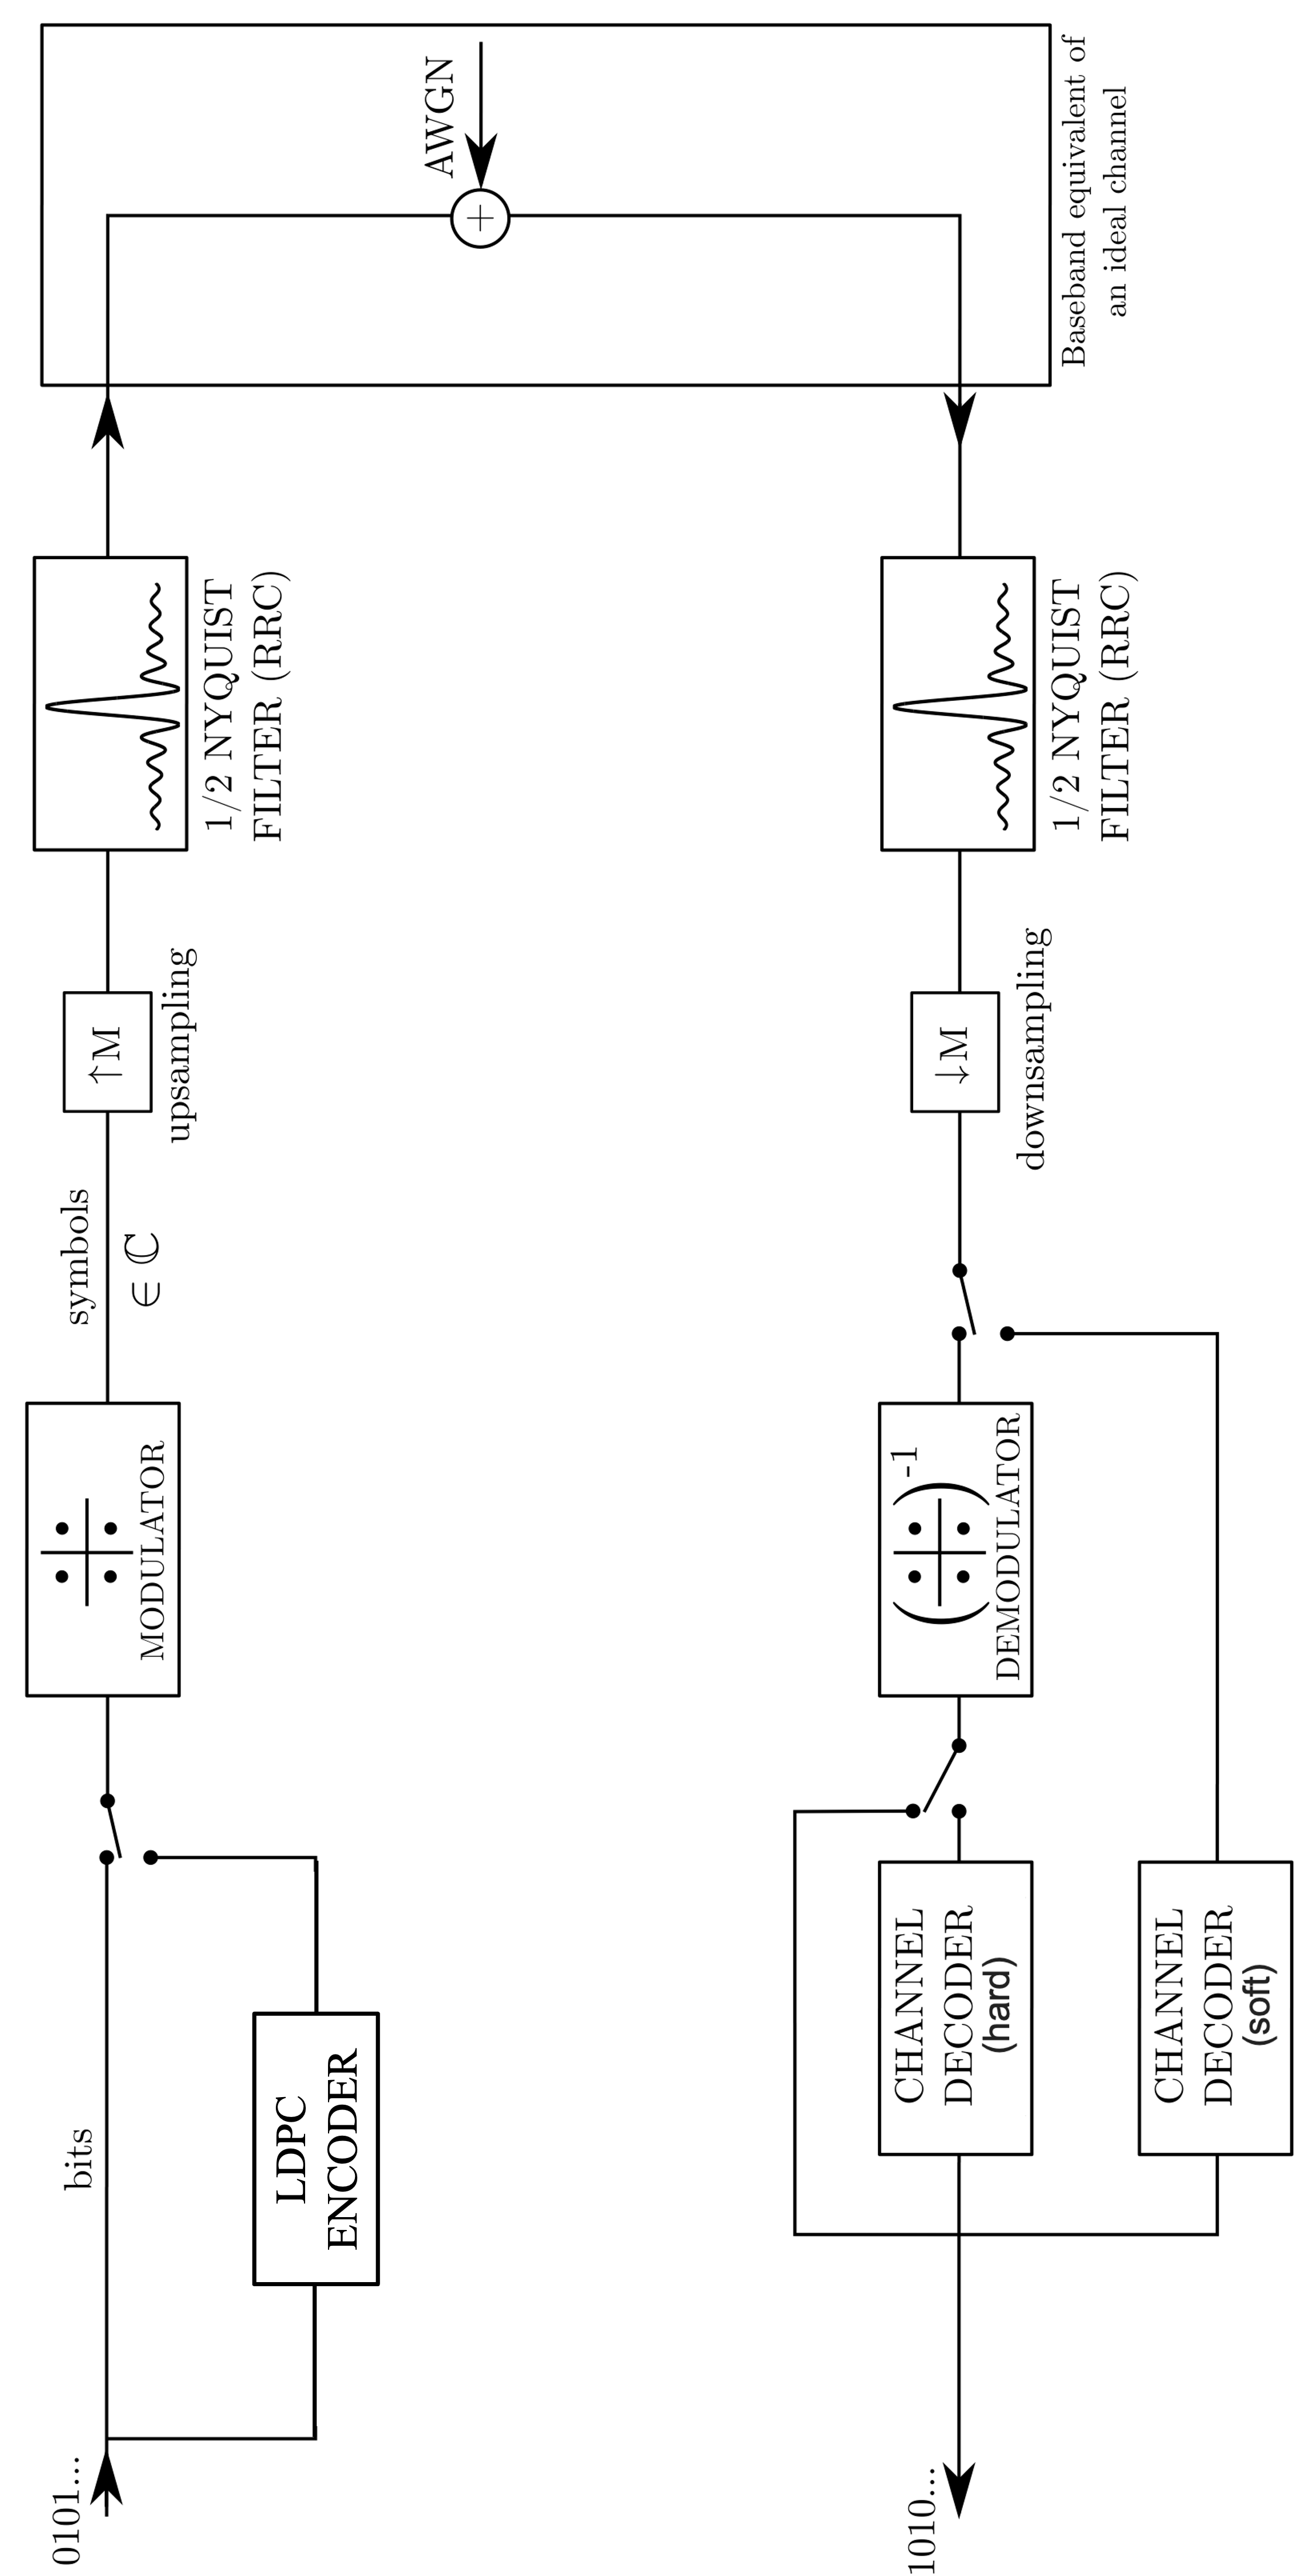
\includegraphics[angle=-90, width=0.7\linewidth]{Images/com-chain}
		\caption{Block diagram of the communication system.}
		\label{fig:com-chain}
	\end{figure}
	Figure \ref{fig:com-chain} shows the simulated DVB-C baseband communication chain. A transmitter generates a bit-stream, maps it to QAM symbols, up-samples, and shapes them with a half-root Nyquist filter to limit bandwidth. The receiver employs a matched half-root Nyquist filter to maximize SNR, then down-samples at symbol instances, and demapps samples to estimate the transmitted bit-stream.
	\par
	In this project, the Low Density Parity Check Encoder is not implemented, and the algorithms for symbol mapping and demapping were provided.
	
	\subsection{Bit Generation and Symbol Mapping and Demapping}
	Mapping bit-streams to complex symbols enhances spectral efficiency (more bits/symbol per bandwidth). Symbol demapping in the receiver estimates the bit sequence from noisy symbols using the Maximum Likelihood (ML) criterion. ML selects the constellation symbol $\underline{s}_{m}$ minimizing Euclidean distance to the received sample $\underline{r}$:
	\begin{equation}
		\tilde{\underline{s}}_{m}^{ML} = \arg\min_{\underline{s}_{m}} \left(\sum_{k=1}^{K}(r_{k}-s_{mk})^{2}\right)
	\end{equation}
	Where:
	\begin{itemize}
		\item $\tilde{\underline{s}}_{m}^{ML}$ is the estimated symbol using the ML criterion.
		\item $\underline{r} = [r_1, r_2, \dots, r_K]^T$ is the received vector after demodulation.
		\item $\underline{s}_{m} = [s_{m1}, s_{m2}, \dots, s_{mK}]^T$ is the vector representing the $m$-th possible transmitted symbol.
	\end{itemize}
	Minimizing squared Euclidean distance is equivalent to maximizing $\ln p(\underline{r}|\underline{s}_{m})$ for an Additive White Gaussian Noise (AWGN) channel, where $p(\underline{r}|\underline{s}_{m})$ is the conditional probability of receiving vector $\underline{r}$ given symbol $\underline{s}_m$ was sent.
	
	\subsection{Nyquist Filtering}
	Mapped complex symbols $I[k]$ are up-sampled by OSF $> 1$ and passed through a pulse shaping filter $g(t)$ to:
	\begin{enumerate}
		\item Limit transmitted signal bandwidth.
		\item Control inter-symbol interference.
	\end{enumerate}
	
	\subsubsection{Half-Root Nyquist Filter Design and Matched Filtering}
	For optimal ISI cancellation and SNR maximization, a root-raised cosine (RRC) filter $g(t)$ is used for pulse shaping. The receiver uses a matched filter $g^*(-t)$. Their convolution, $h(t) = g(t) \otimes g^*(-t)$, is the overall channel response, designed to satisfy the Nyquist zero ISI criterion at sampling intervals $T_{symb}$ (normalized $h(t)$):
	\begin{equation}
		h(kT_{symb}) = \begin{cases}
			1 & k=0 \\
			0 & k \neq 0
		\end{cases}
		\label{eq:nyquist_criterion_part1}
	\end{equation}
	\par
	The RRC filter $g(t)$ is derived from a raised-cosine (RC) filter with transfer function $H(f)$. The RRC frequency response is $G(f) = \sqrt{H(f)}$, and $g(t) = \mathcal{F}^{-1}\{G(f)\}$. $H(f)$ is given by:
	\begin{equation}
		H(f) = \begin{cases}
			T_{symb} & 0 \le |f| < \frac{1-\beta}{2T_{symb}} \\ 
			\frac{T_{symb}}{2} \left(1 + \cos\left[\frac{\pi T_{symb}}{\beta}\left(|f| - \frac{1-\beta}{2T_{symb}}\right)\right]\right) & \frac{1-\beta}{2T_{symb}} \le |f| \le \frac{1+\beta}{2T_{symb}} \\ 
			0 & |f| > \frac{1+\beta}{2T_{symb}}
		\end{cases}
		\label{eq:rc_response_part1}
	\end{equation}
	
	\subsubsection{Filter Properties and Inter-Symbol Interference Cancellation}
	\begin{figure}[H]
		\centering
		\begin{subfigure}[b]{0.48\textwidth}
			\centering
			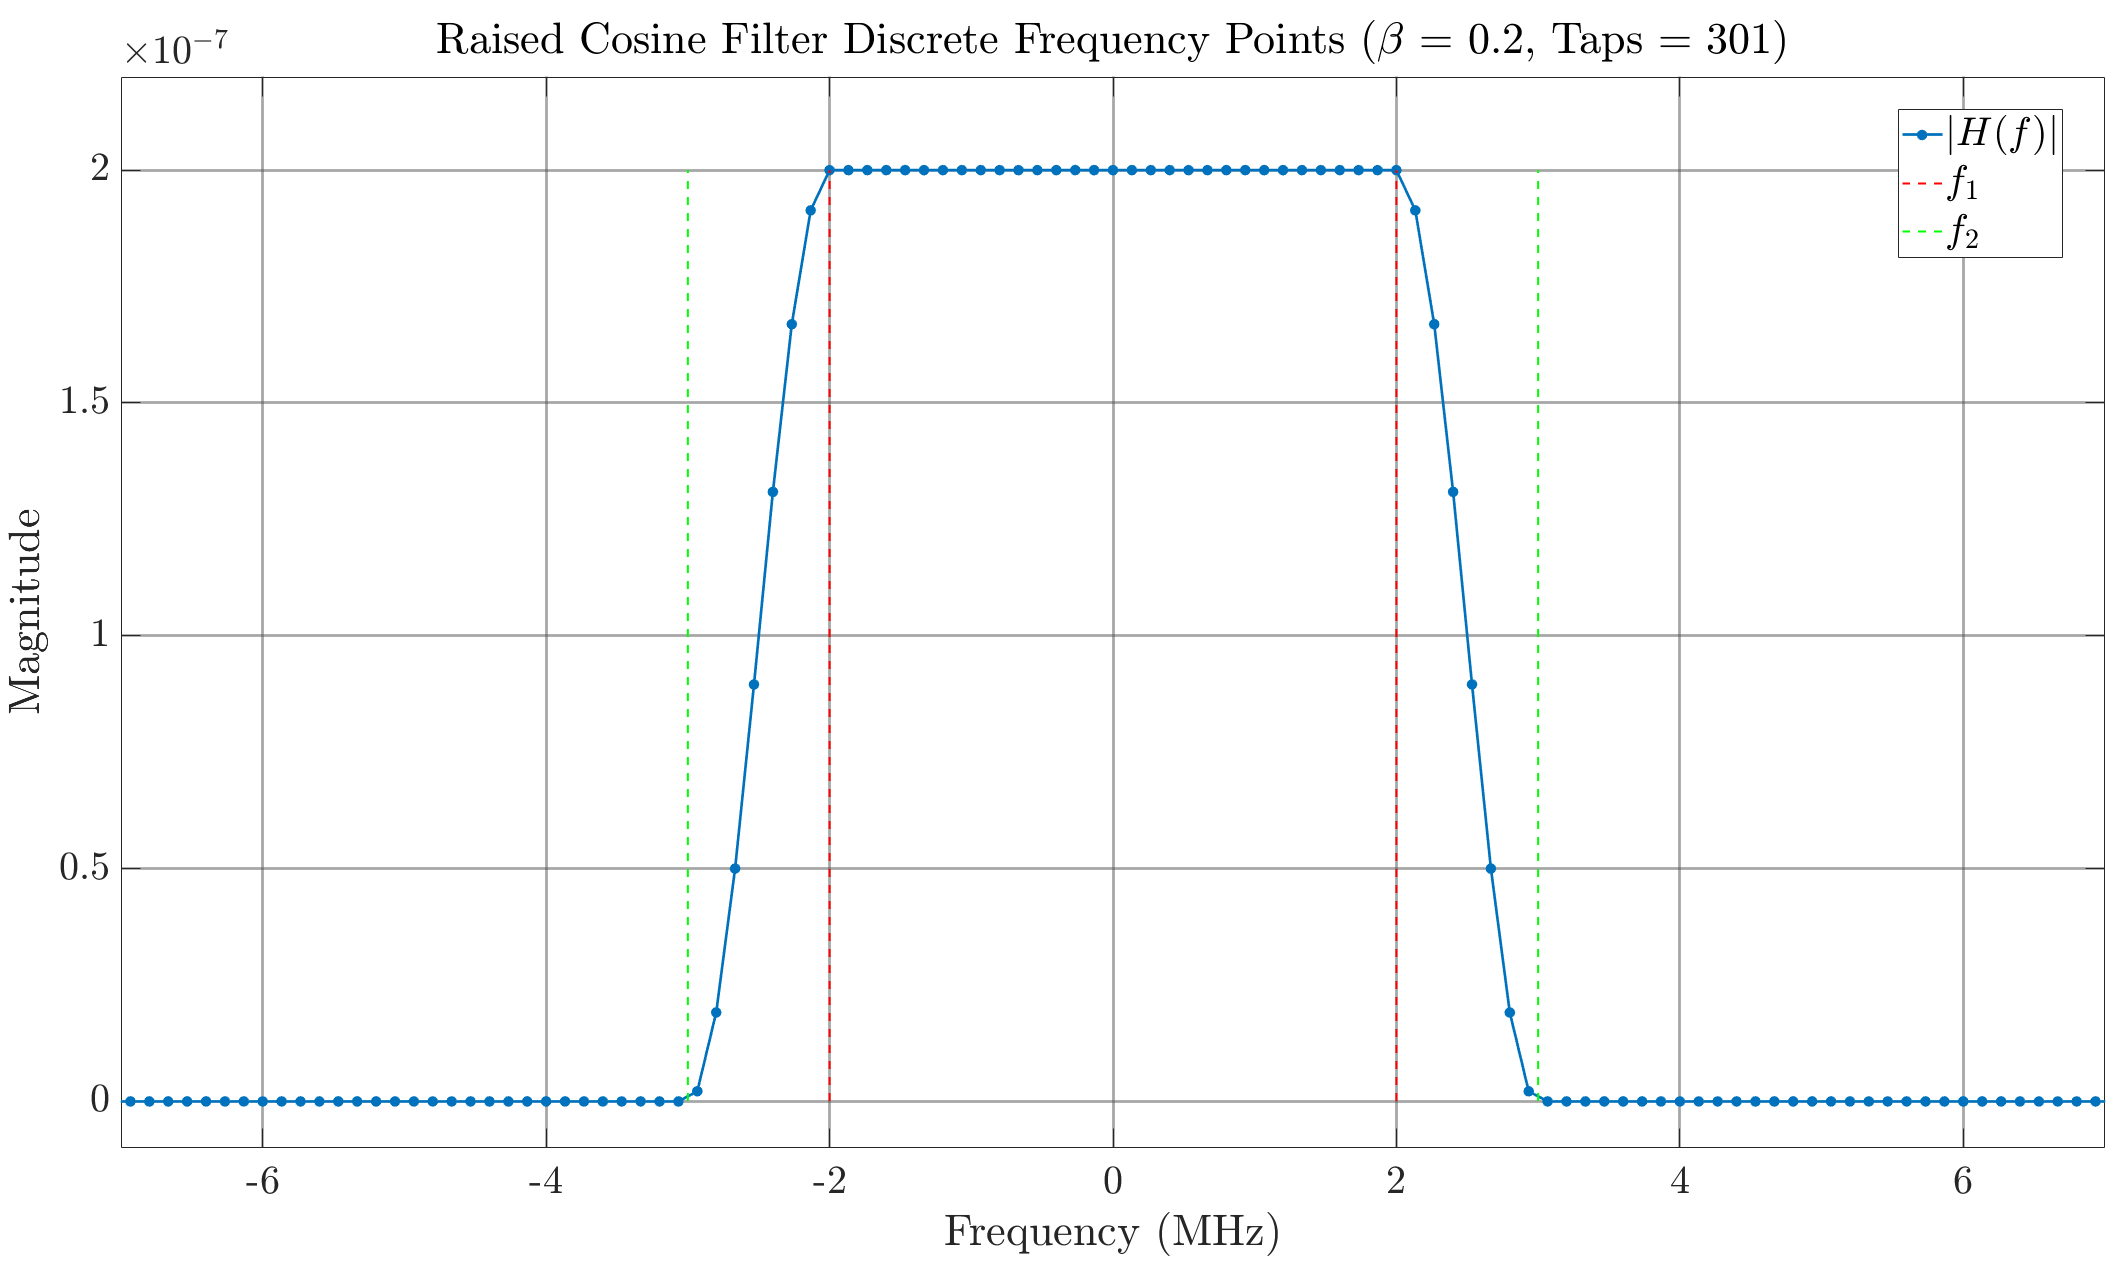
\includegraphics[width=\linewidth]{Images/h-rc-freq}
			\caption{Simulated Raised Cosine Filter Frequency Response from ($\beta = 0.2$, $taps = 301$, $OSF = 8$).}
			\label{fig:h-rc-freq}
		\end{subfigure}
		\hfill % This will add horizontal space between the subfigures
		\begin{subfigure}[b]{0.48\textwidth}
			\centering
			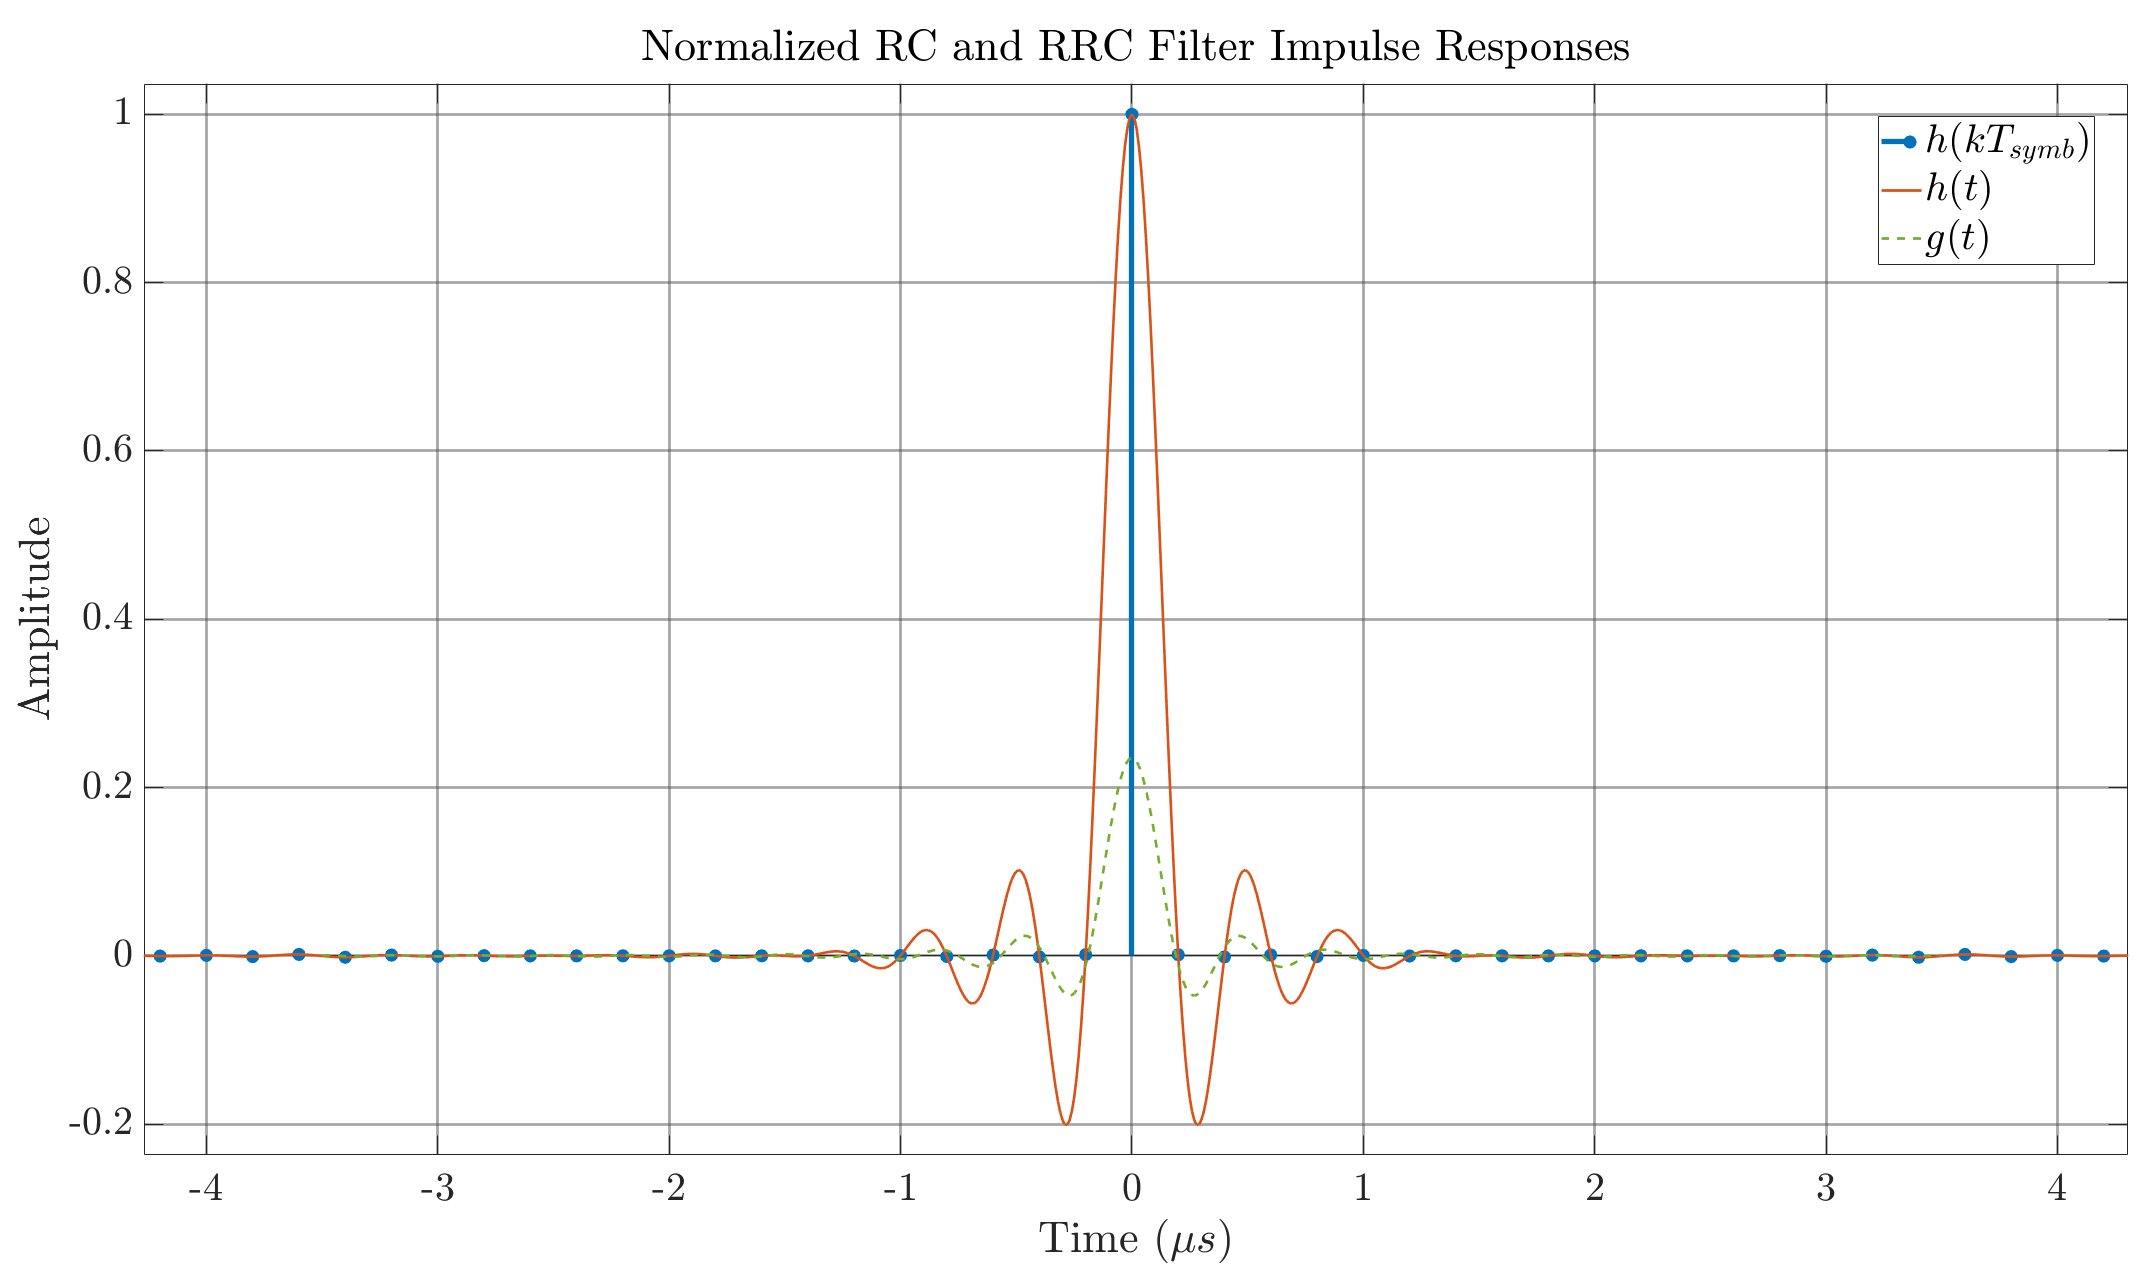
\includegraphics[width=\linewidth]{Images/h-rc}
			\caption{Simulated Normalized RC and RRC filter Impulse Responses, with $h(kT_{symb})$ illustrating ISI cancellation.}
			\label{fig:h-rc}
		\end{subfigure}
		\caption{Simulated characteristics of the Nyquist filtering: frequency response (left) and impulse responses (right).}
		\label{fig:nyquist-filter-combined}
	\end{figure}
	
	The overall RC filter $h(t)$ confines signal energy to bandwidth $B = R_{symb} (1+\beta)/2$, where $R_{symb} = 1/T_{symb}$. Figure \ref{fig:h-rc-freq} shows the simulated $H(f)$ (from Eq. \ref{eq:rc_response_part1}), confirming spectral confinement with its passband, roll-off, and stopband. For project parameters ($R_{symb} = !!!!!!!!!!$ and $\beta = 0.2$), $B = 0.6 R_{symb}$.
	
	In the time domain, $h(t)$ when sampled at $T_{symb}$ intervals approximates a Dirac delta, satisfying Eq. \ref{eq:nyquist_criterion_part1} for zero ISI. Figure \ref{fig:h-rc} shows the simulated $h(t)$; stems at $h(kT_{symb})$ (unity at $t=0$, zero elsewhere) confirm ISI elimination by nullifying other symbols' contributions at the optimal sampling instant.
	
	
	\subsection{Noise Addition and Performance Evaluation}
	AWGN, representing cumulative interference and thermal noise, limits performance. In the simulated baseband model, the received signal $r(t)$ is $s(t)$ (output of $g(t)$) plus complex baseband noise $n(t)$:
	\begin{equation}
		r(t) = s(t) + n(t)
	\end{equation}
	\par
	The noise $n(t)$ is complex Gaussian, with independent real/imaginary components, each with Power Spectral Density (PSD) $N_0/2$. After matched filtering with $g^*(-t)$ and sampling at $t = kT_{symb}$, the $k$-th received sample is $y[k] = (r(t) \otimes g^*(-t))|_{t=kT_{symb}}$. Since the signal component of $r(t)$ is $\sum_m I[m]g(t-mT_{symb})$, and $h(t) = g(t) \otimes g^*(-t)$ satisfies the Nyquist criterion (Eq. \ref{eq:nyquist_criterion_part1}, with $h(0)$ normalized to 1):
	\begin{align}
		y[k] &= \left( \left(\sum_m I[m]g(t-mT_{symb})\right) \otimes g^*(-t) \right)\Big|_{t=kT_{symb}} + (n(t) \otimes g^*(-t))|_{t=kT_{symb}} \nonumber \\
		&= \sum_m I[m]h((k-m)T_{symb}) + n_o[k] \nonumber \\
		&= I[k]h(0) + \sum_{m \neq k} I[m]h((k-m)T_{symb}) + n_o[k] \nonumber \\
		&= I[k] + n_o[k] \label{eq:yk_plus_noise}
	\end{align}
	where $I[k]$ is the transmitted complex symbol and $n_o[k] = (n(t) \otimes g^*(-t))|_{t=kT_{symb}}$ is the filtered and sampled noise. The noise samples $n_o[k]$ are complex Gaussian, as $n(t)$ is white Gaussian and matched filtering is linear. Real/imaginary components of $n_o[k]$ are independent, each with variance $\sigma^2 = N_0/2$.
	
	System performance is evaluated by simulating Bit Error Rate (BER) vs. $E_b/N_0$, based on Eq. \ref{eq:yk_plus_noise}. To simulate at a specific $E_b/N_0$, noise power $n_o[k]$ is set relative to signal power. Average symbol energy $E_s = \text{E}\left[|I[k]|^2\right]$. Average bit energy $E_b = E_s / b = E_s / \log_2 M$ (M-QAM, $b$ bits/symbol). Then, $N_0 = E_b / (E_b/N_0)_{\text{target}}$. The complex noise $n_o[k]$ added per Eq. \ref{eq:yk_plus_noise} has total variance $N_0$ (real/imaginary components each $N_0/2$).
	
	Experimental BER is:
	\begin{equation}
		\text{BER}_{\text{exp}} = \frac{\text{Number of erroneously detected bits}}{\text{Total number of transmitted bits}}
	\end{equation}
	Simulated BER vs. $E_b/N_0$ is compared to theoretical $P_b$ for M-QAM (square, Gray coded, moderate/high $E_b/N_0$):
	\begin{equation}
		P_b \approx \frac{4}{\log_2 M} \left(1 - \frac{1}{\sqrt{M}}\right) Q\left(\sqrt{\frac{3 (\log_2 M)}{M-1} \frac{E_s}{N_0}}\right) = \frac{4}{\log_2 M} \left(1 - \frac{1}{\sqrt{M}}\right) Q\left(\sqrt{\frac{3 (\log_2 M)^2}{M-1} \frac{E_b}{N_0}}\right)
		\label{eq:Pb_MQAM_Eb_cont_final}
	\end{equation}
	where $Q(x) = \frac{1}{\sqrt{2\pi}} \int_x^\infty e^{-u^2/2} du$.
	
	Figure \ref{fig:ber-mod_cont} shows simulated BER for various QAMs, illustrating the spectral vs. power efficiency trade-off: higher-order modulations offer higher data rates but need more power for the same BER.
	
	\begin{figure}[H]
		\centering
		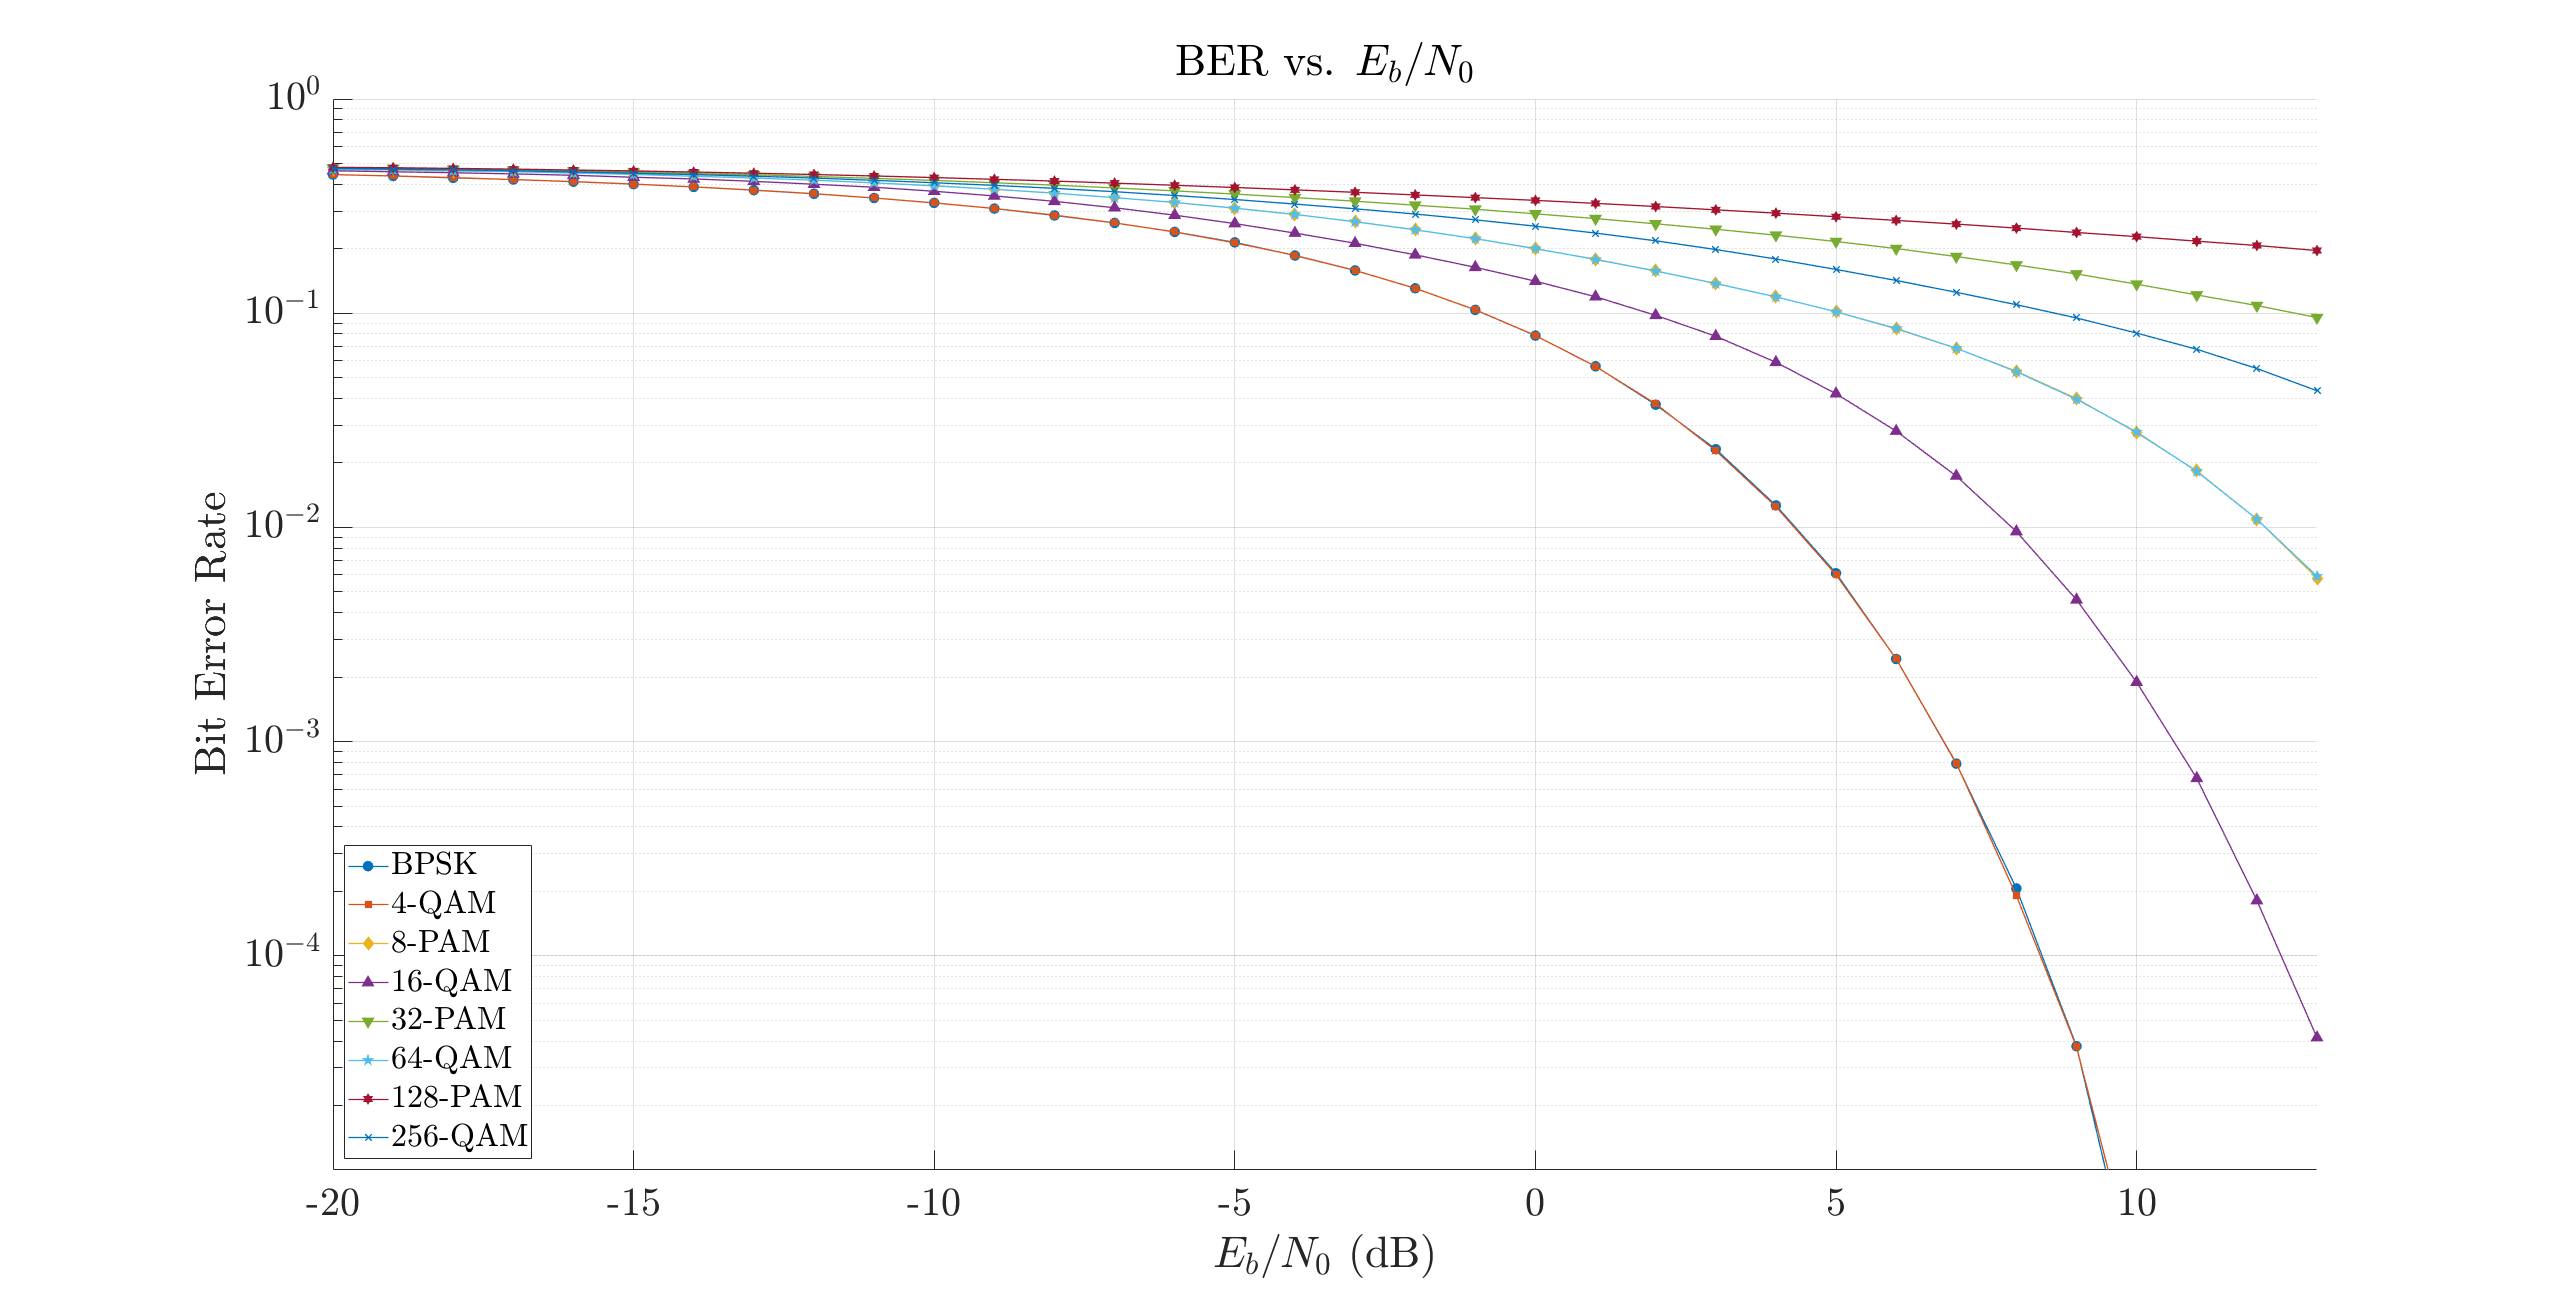
\includegraphics[width=0.8\linewidth]{Images/ber-mod.png}
		\caption{Simulated BER vs. $E_b/N_0$ for various modulation types}
		\label{fig:ber-mod_cont}
	\end{figure}
	
	Figure \ref{fig:constellations-noise_cont} shows AWGN's effect on 16-QAM constellations. Figure \ref{fig:const-noisy_cont} displays symbols $s(t)+n(t)$ pre-matched filter. Post-matched filtering and downsampling ($y[k]=I[k]+n_o[k]$), symbols in Fig. \ref{fig:const-filtered-down_cont} cluster around ideal points, validating the matched filter's SNR maximization.
	
	\begin{figure}[H]
		\centering
		\begin{subfigure}{0.48\textwidth}
			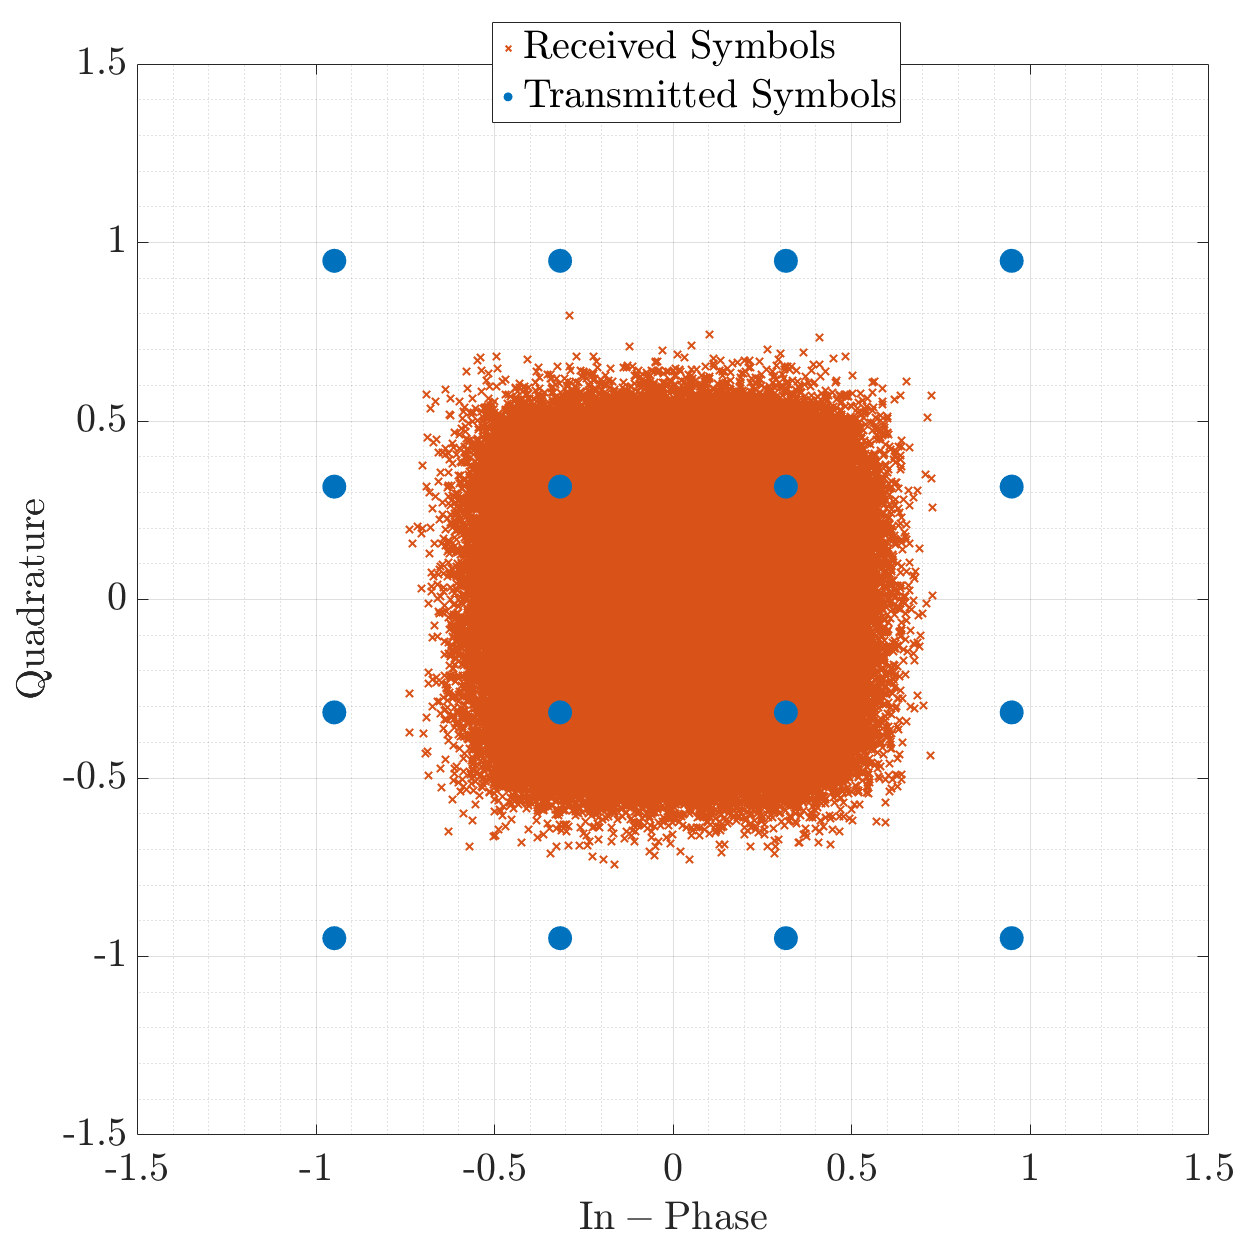
\includegraphics[width=\linewidth]{Images/const-noisy.png}
			\caption{Simulated noisy 16-QAM symbols before matched filter.}
			\label{fig:const-noisy_cont}
		\end{subfigure}\hfill
		\begin{subfigure}{0.48\textwidth}
			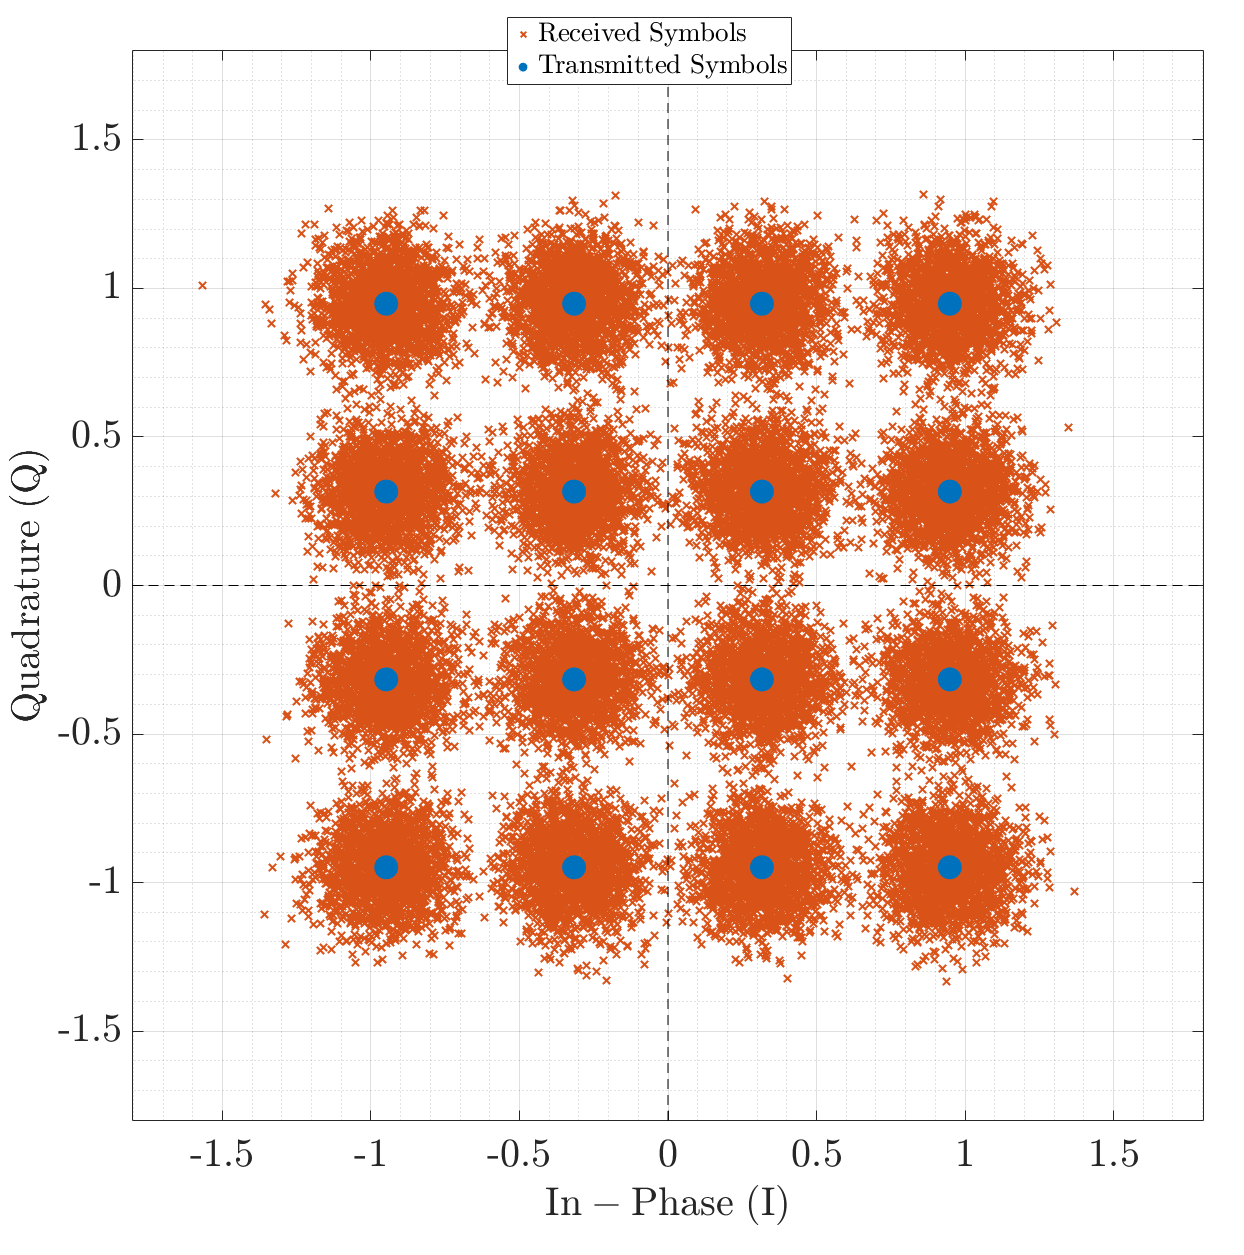
\includegraphics[width=\linewidth]{Images/const-filtered-down.png} 
			\caption{Simulated 16-QAM symbols after matched filtering and downsampling.}
			\label{fig:const-filtered-down_cont}
		\end{subfigure}
		\caption{Simulation - Effect of AWGN and matched filtering on a 16-QAM constellation ($\frac{E_b}{N_0} = 15$ dB)}
		\label{fig:constellations-noise_cont}
	\end{figure}
	
	\section{Time and Frequency Synchronization}
	\subsection{The Problem of Synchronization}
	\begin{figure}[H]
		\centering
		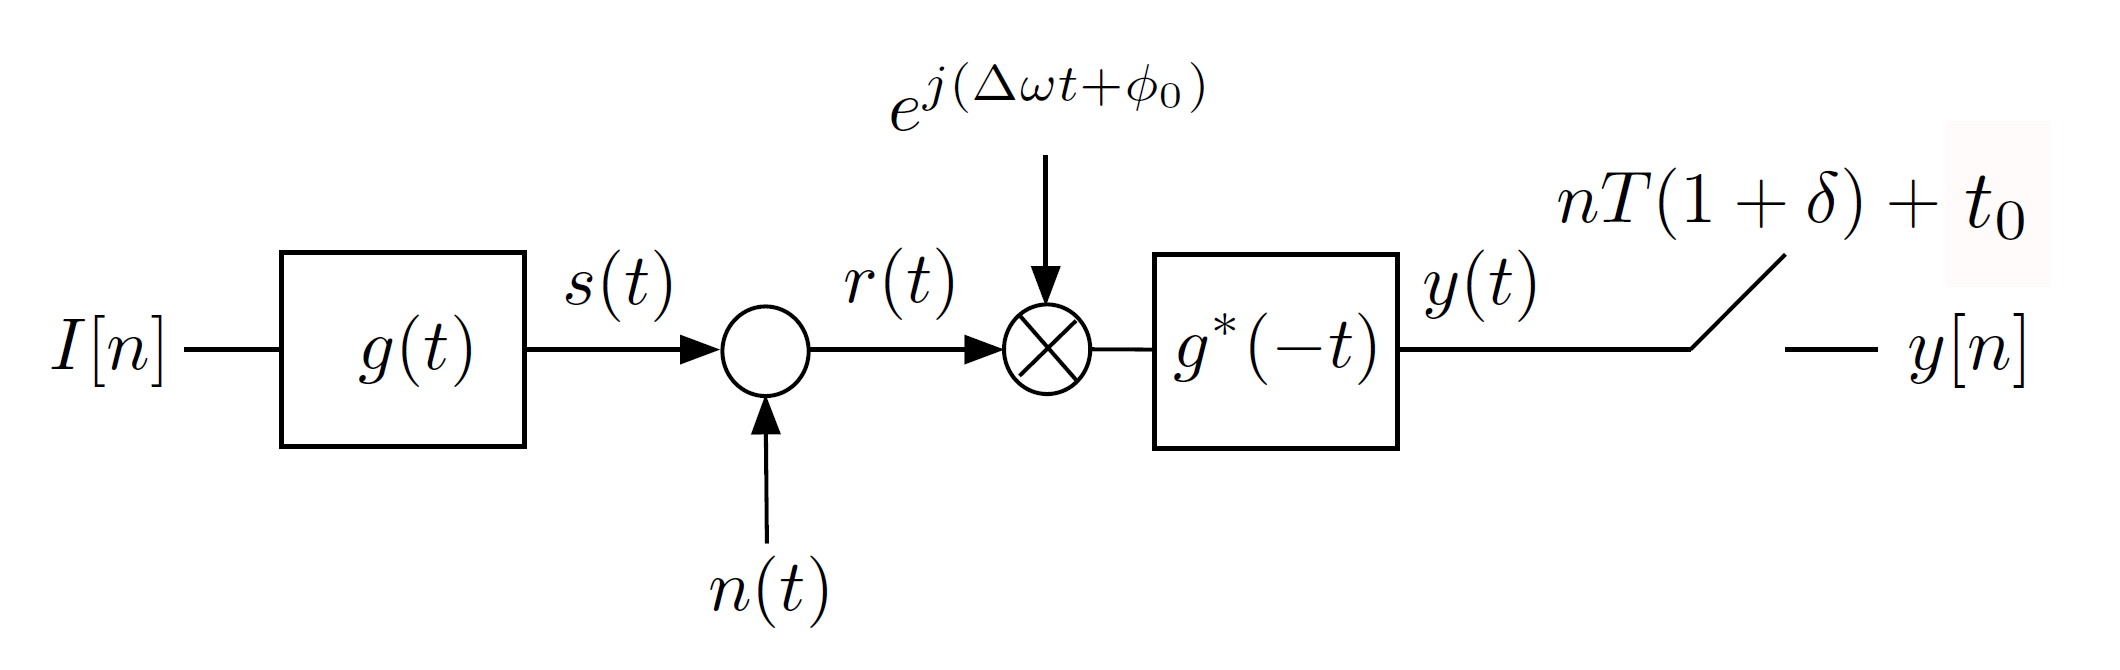
\includegraphics[width=0.8\linewidth]{sync-errors-conceptual} % Path: Images/sync-errors-conceptual
		\caption{Synchronization mismatches at the receiver}
		\label{fig:sync-errors-conceptual}
	\end{figure}
	Accurate demodulation requires transmitter-receiver synchronization: precise symbol sampling instances and carrier frequency/phase alignment. Errors stem from independent local oscillators (frequency deviations from manufacturing/environment) and propagation delay (unknown phase shift, timing offset).
	\par
	Key synchronization errors:
	\begin{itemize}
		\item Carrier Frequency Offset (CFO), $\Delta f$: Difference between transmitter's and receiver's carrier frequencies.
		\item Carrier Phase Offset, $\phi_0$: Phase difference between incoming carrier and receiver's local oscillator.
		\item Sample Clock Offset (SCO), $\delta$: Frequency mismatch between transmitter's DAC clock and receiver's ADC clock (considered negligible and not implemented).
		\item Sample Time Shift, $t_0$: Receiver's uncertainty about symbol arrival time, necessitating optimal sampling instant determination.
	\end{itemize}
	Figure \ref{fig:sync-errors-conceptual} illustrates these mismatches: symbols generated at $nT_{symb}$ are effectively sampled at $nT_{symb}(1+\delta)+t_0$ by the receiver.
	
	
	\subsection{Impact of Synchronization Errors on Performance}
	\subsubsection{Impact of Carrier Phase Offset ($\phi_0$)}
	A static carrier phase offset $\phi_0$ (phase difference between incoming carrier and local oscillator) rotates the received constellation by $\phi_0$. With perfect timing, no CFO, and no noise, a transmitted symbol $I[n]$ becomes at matched filter output:
	\begin{equation}
		y[n] = I[n]e^{j\phi_0}
	\end{equation}
	\par
	Uncorrected rotation causes detection errors.
	
	\subsubsection{Impact of Carrier Frequency Offset ($\Delta f$)}
	\begin{figure}[H]
		\centering
		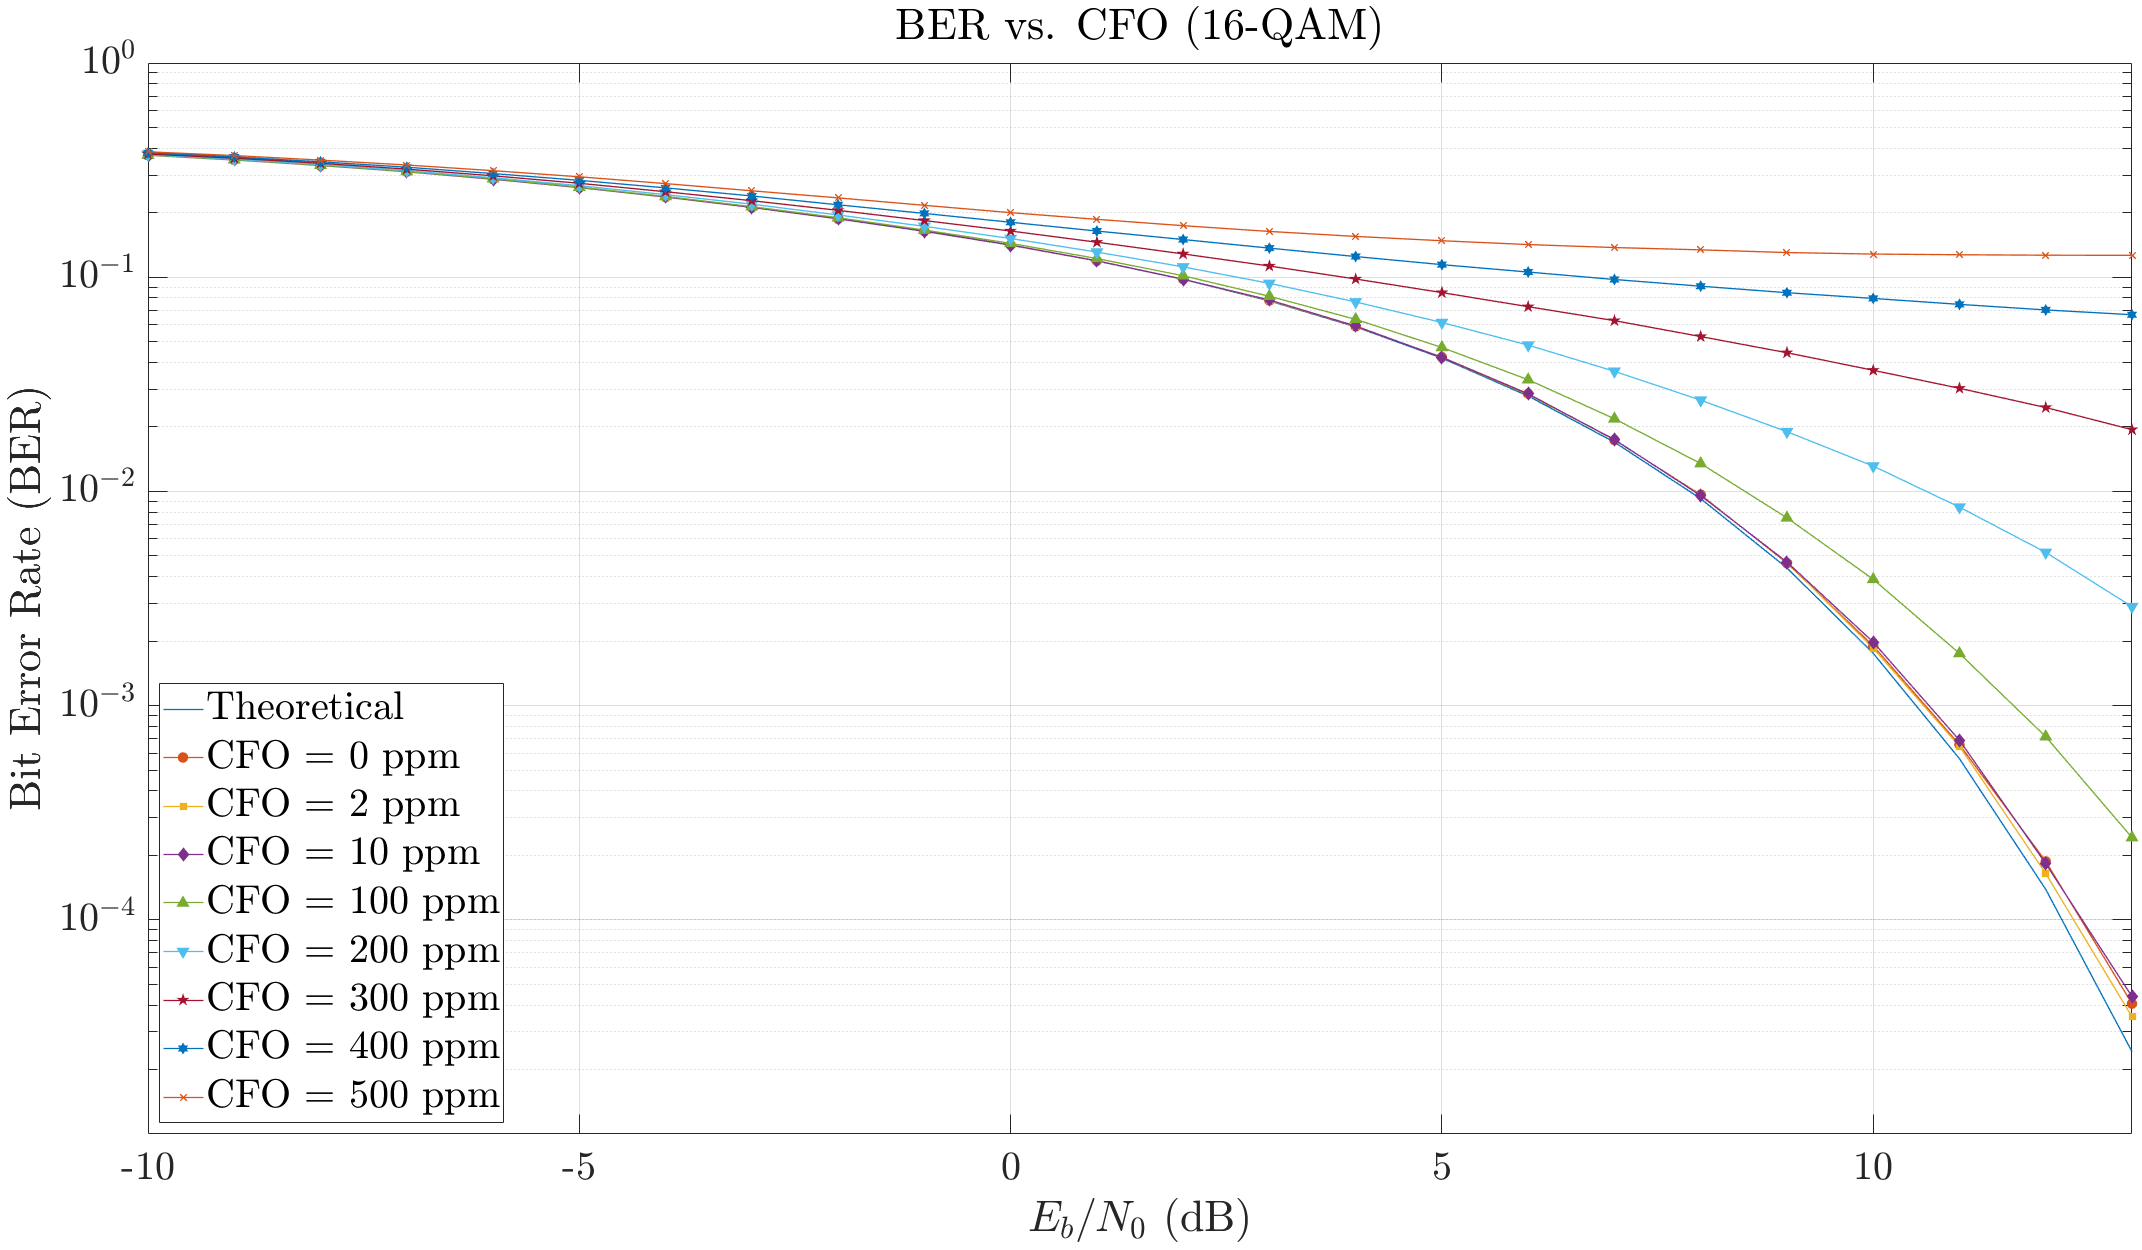
\includegraphics[width=0.8\linewidth]{ber-cfo}
		\caption{Simulated BER vs. $E_b/N_0$ for 16-QAM with varying CFO}
		\label{fig:ber-cfo}
	\end{figure}
	With CFO $\Delta f$, the pre-matched filter signal is $r(t) = s(t) e^{j(2\pi \Delta f t)}$ (no noise/phase offset). Impacts:
	\begin{enumerate}
		\item Phase Drift: Sampled symbols $y[n] = I[n] e^{j(2\pi \Delta f nT_{symb})}$ experience progressive phase rotation, causing constellation points to form circles. Fig. \ref{fig:cfo-po-sub} (16-QAM, $E_b/N_0=15$ dB) shows symbols smeared along arcs due to this and an initial phase offset.
		\item Inter-Symbol Interference: Significant CFO shifts the signal spectrum, misaligning $g^*(-t)$ with $g(t)e^{j2\pi \Delta f t}$, causing SNR loss and ISI. Fig. \ref{fig:ber-cfo} (16-QAM) quantifies BER degradation. E.g., 100 ppm CFO needs ~2 dB more $E_b/N_0$ for BER $10^{-3}$. Higher CFO worsens performance (more ISI, phase drift).
	\end{enumerate}
	
	\subsubsection{Impact of Sample Time Shift ($t_0$)}
	\begin{figure}[H]
		\centering
		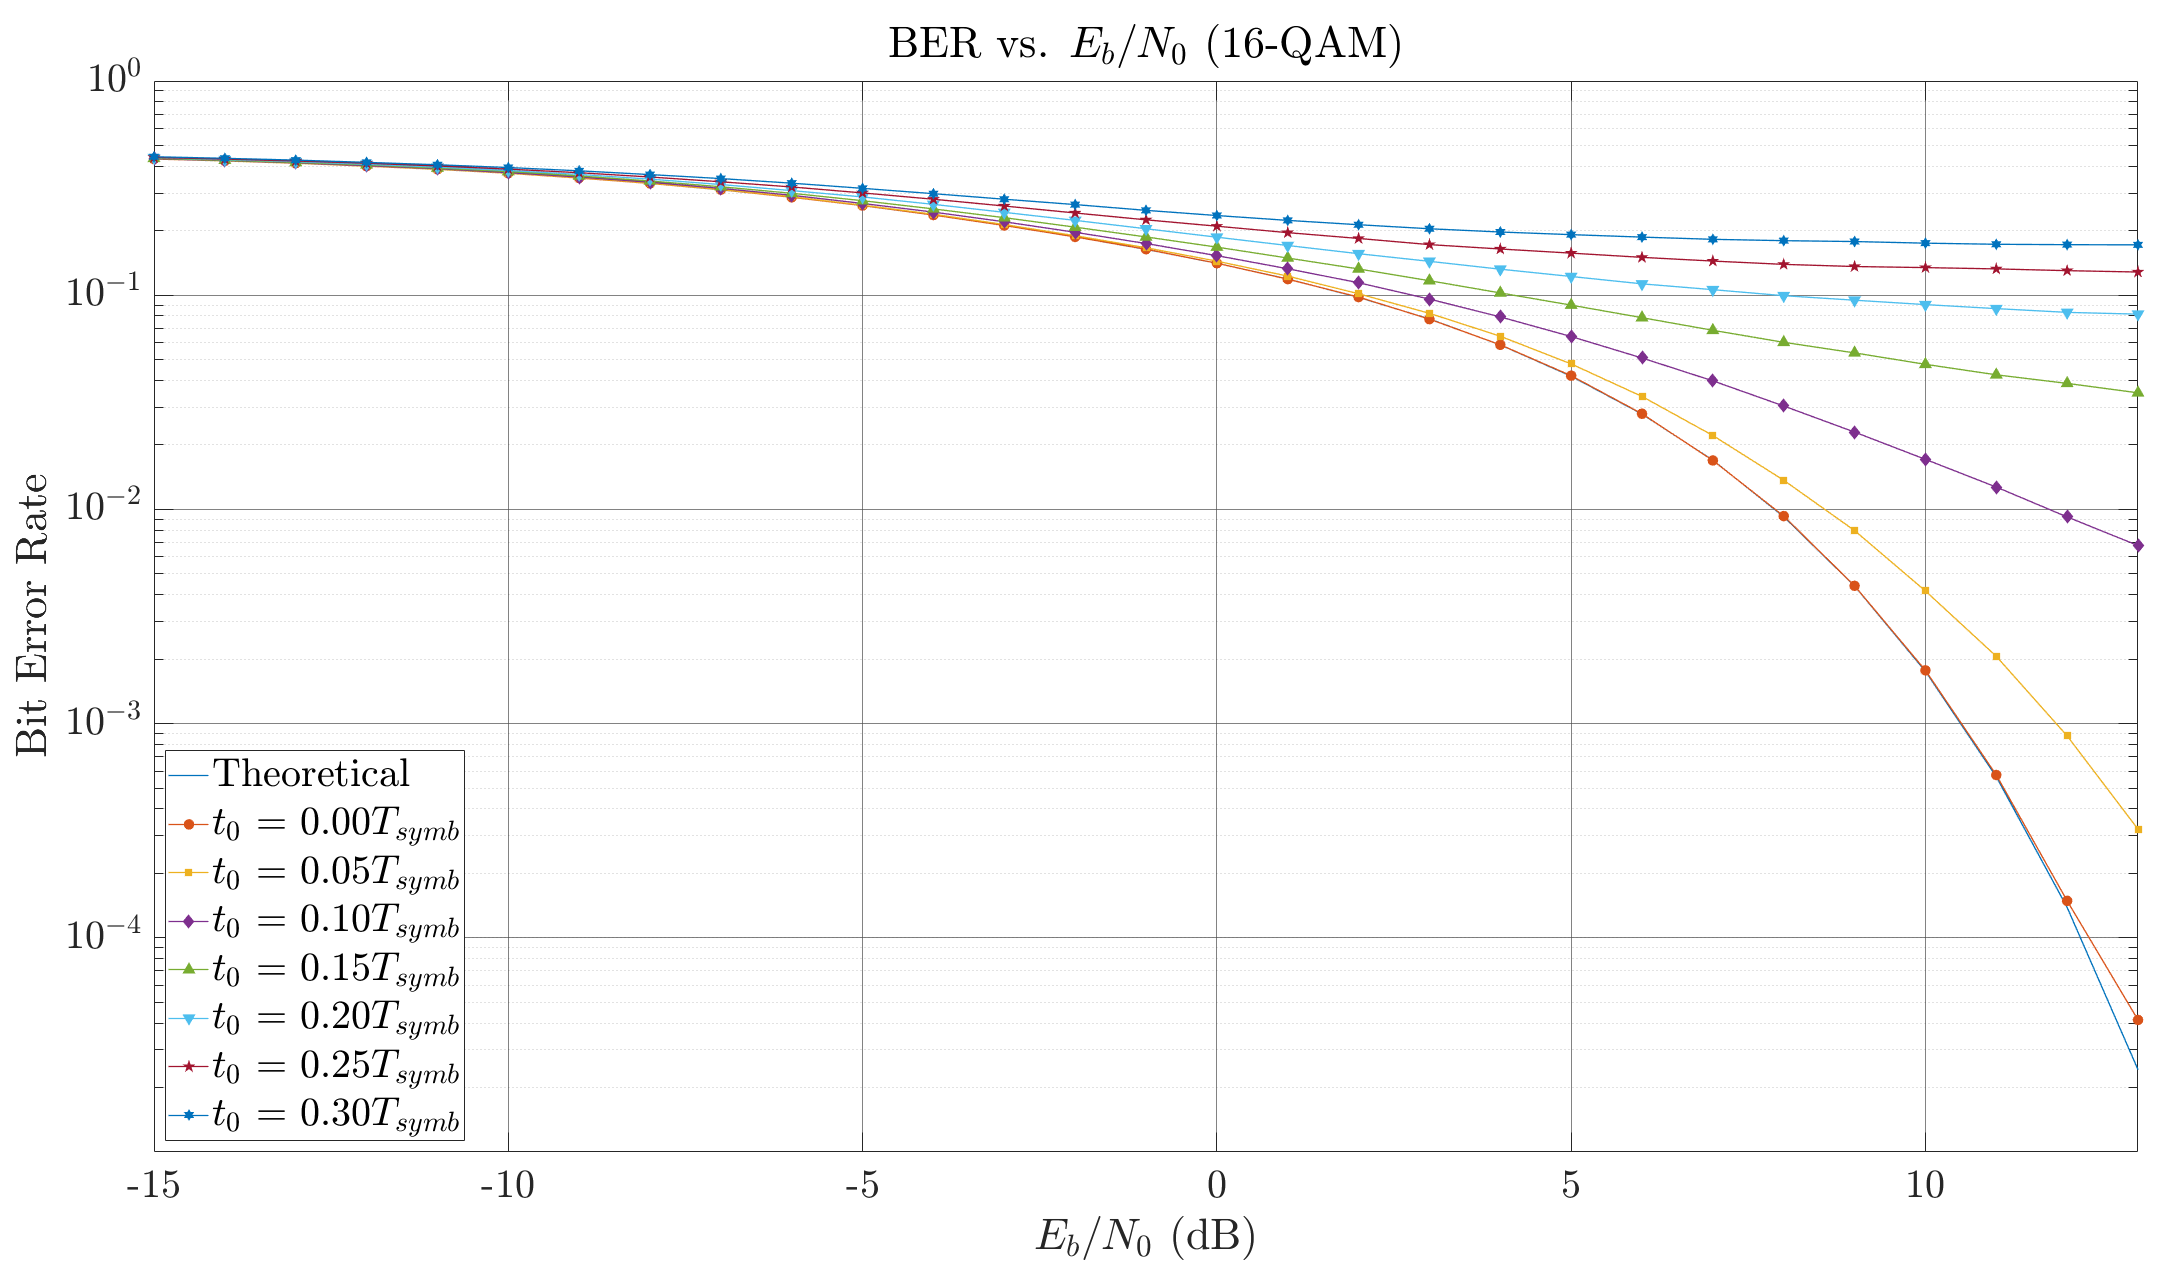
\includegraphics[width=0.8\linewidth]{ber-timing}
		\caption{Simulated BER vs. $E_b/N_0$ for 16-QAM with varying timing offsets}
		\label{fig:ber-timing}
	\end{figure}
	An incorrect sampling instant $t_0 \neq 0$ (vs. optimal) means sampling off maximum signal energy and zero ISI point. For Nyquist filter $h(t)$ (no noise), sampling at $nT_{symb} + t_0$ yields:
	\begin{align}
		y[n] &= \sum_m I[m]h((n-m)T_{symb} + t_0) \\
		&= I[n]h(t_0) + \sum_{m \neq n} I[m]h((n-m)T_{symb} + t_0) \label{eq:timing_offset_impact_revised}
	\end{align}
	\par
	The term $I[n]h(t_0)$ is the attenuated symbol ($h(t_0) < h(0)$ for $t_0 \neq 0$). The sum is ISI ($h(kT_{symb} + t_0) \neq 0$ for $k \neq 0, t_0 \neq 0$). Fig. \ref{fig:ber-timing} (16-QAM) shows BER degradation: increasing $t_0$ from $0 T_{symb}$ to $0.3 T_{symb}$ progressively worsens BER.
	
	\begin{figure}[H]
		\centering
		\begin{subfigure}[b]{0.48\textwidth}
			\centering
			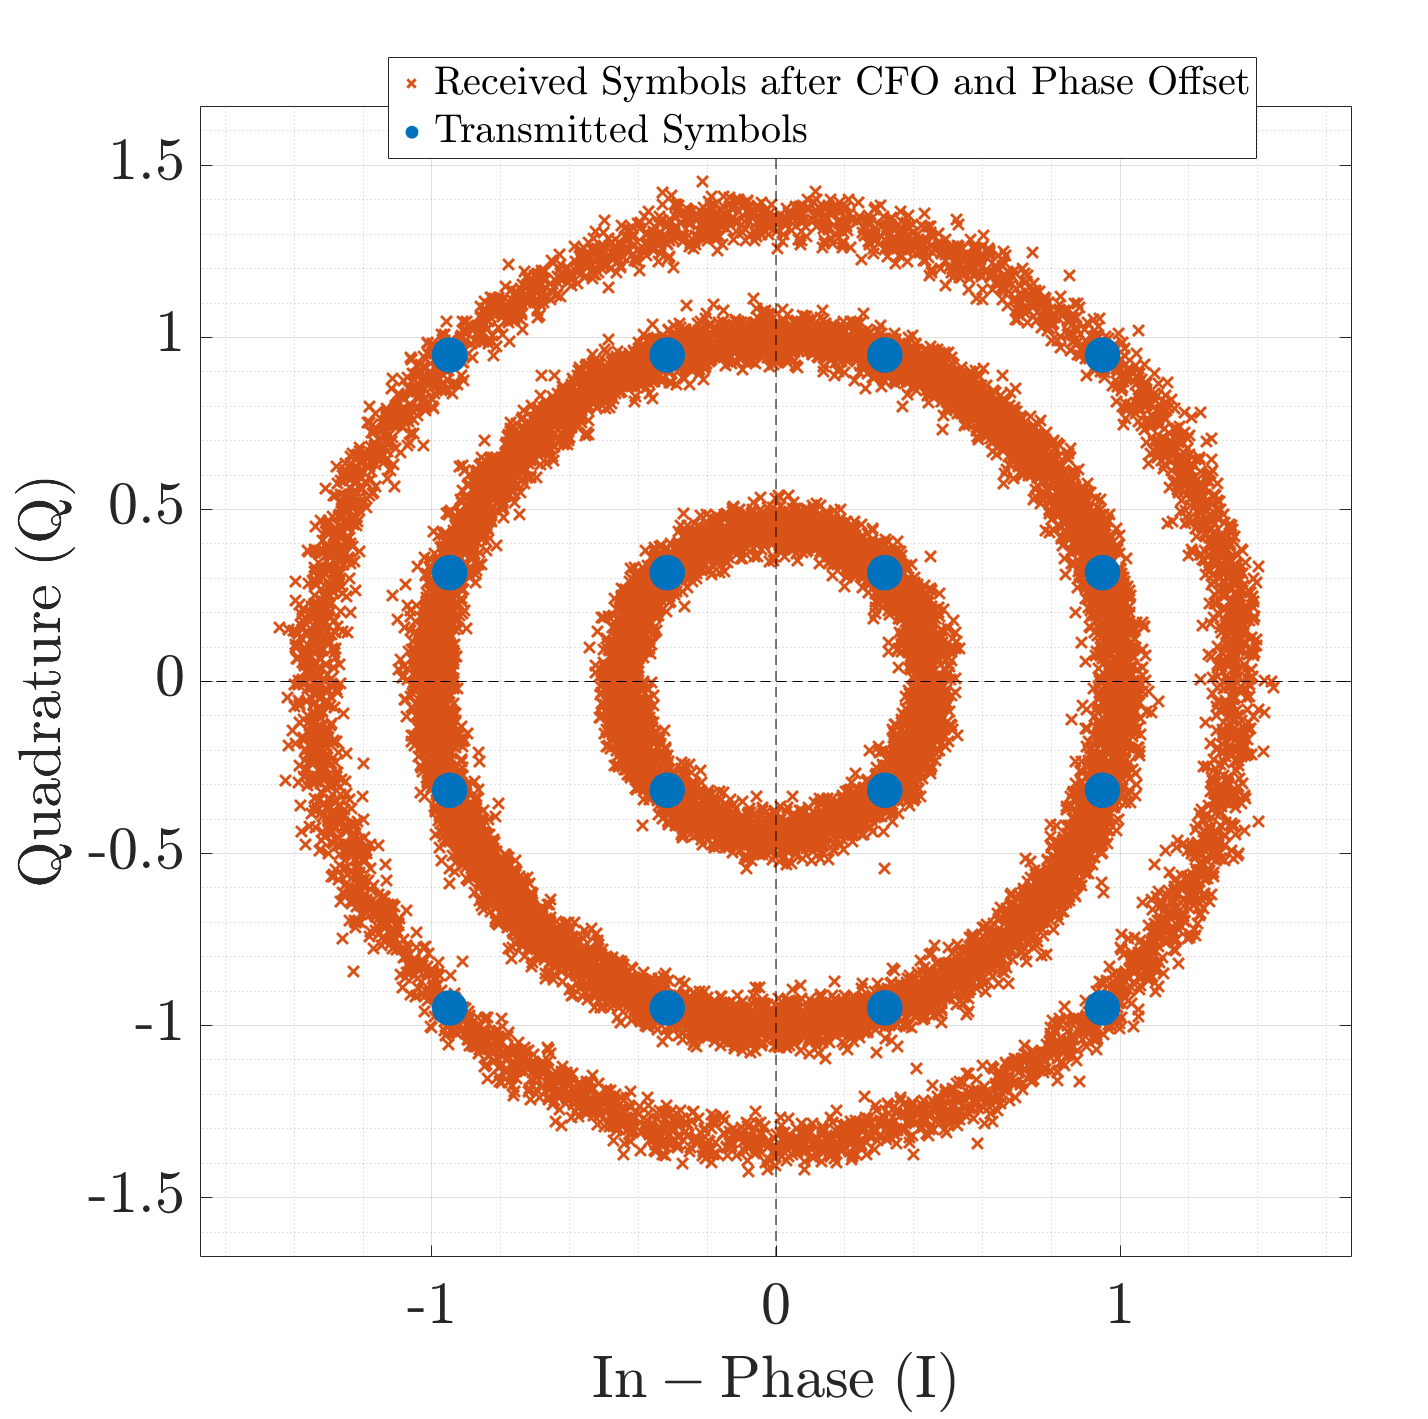
\includegraphics[width=\linewidth]{cfo-po}
			\caption{16-QAM Constellation diagram after CFO and Phase Offset}
			\label{fig:cfo-po-sub}
		\end{subfigure}
		\hfill 
		\begin{subfigure}[b]{0.48\textwidth}
			\centering
			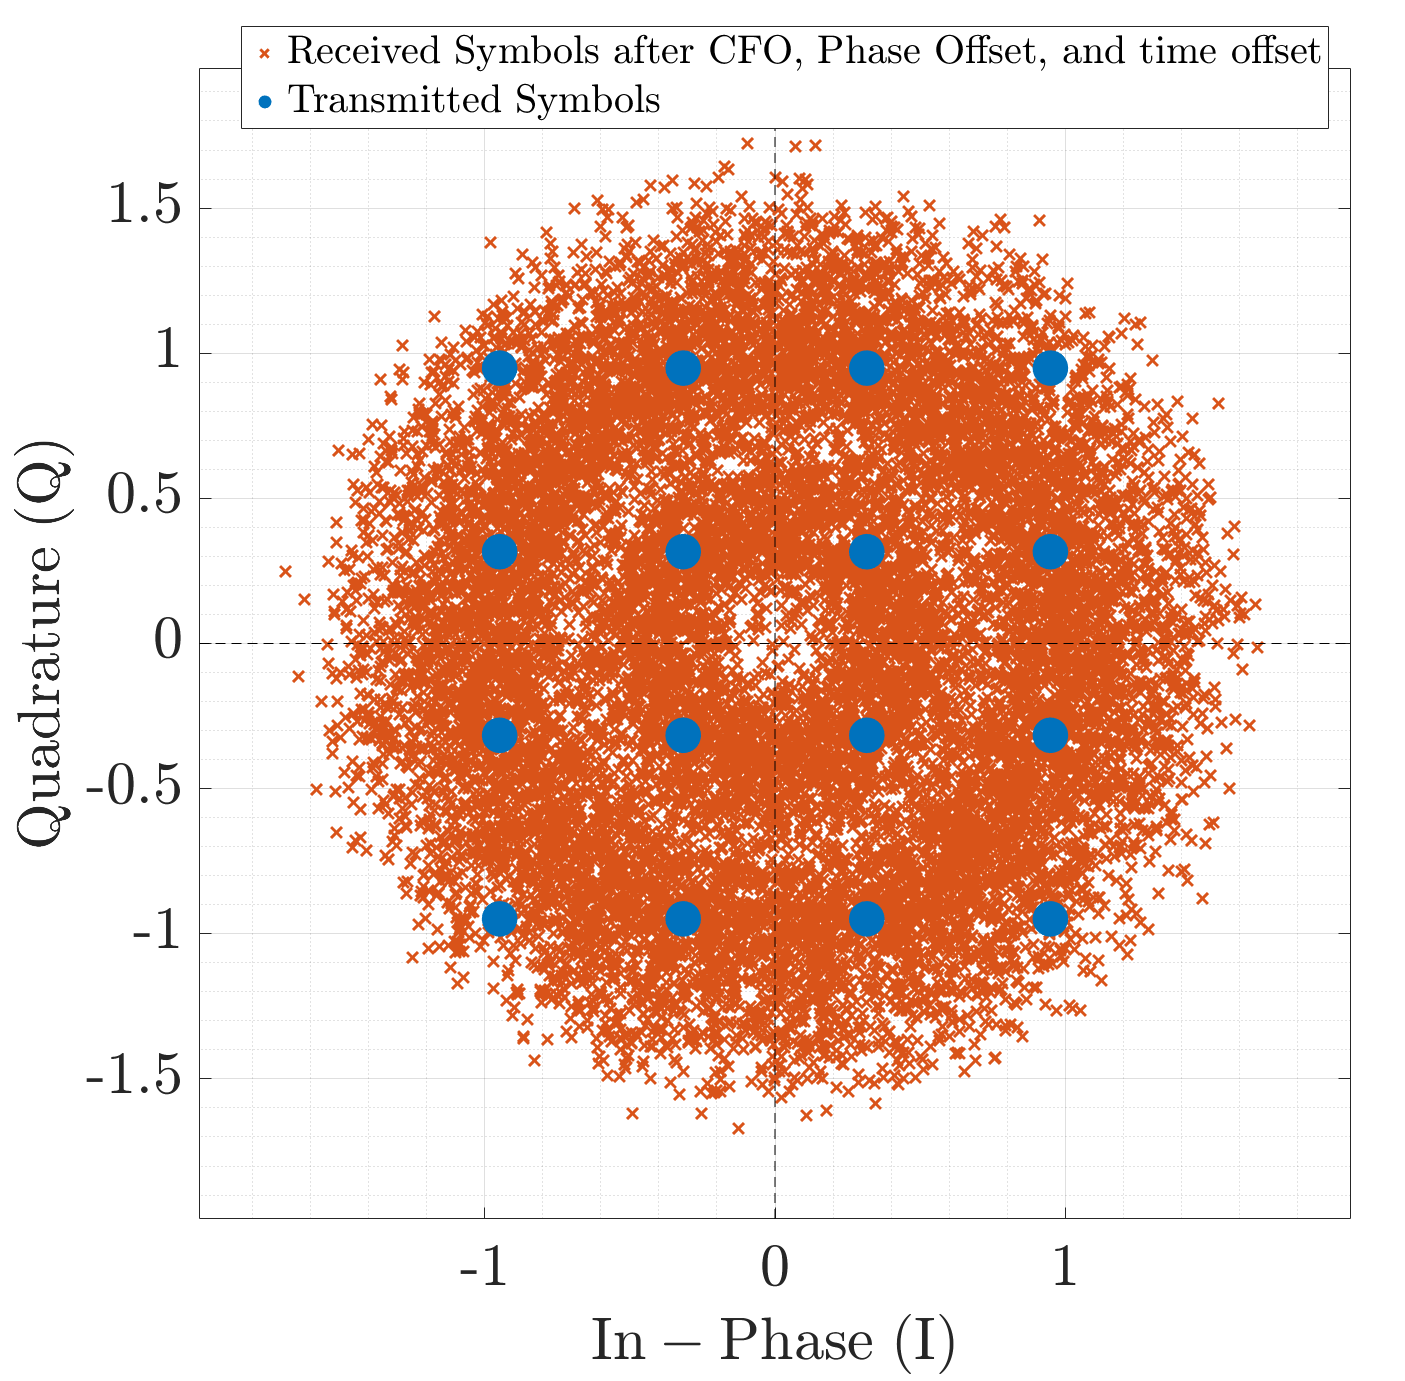
\includegraphics[width=\linewidth]{cfo-po-to}
			\caption{16-QAM Constellation diagram after CFO, Phase Offset and time offset}
			\label{fig:cfo-po-to-sub}
		\end{subfigure}
		\caption{Simulated Constellation diagrams of symbols transmitted and received after adding AWGN noise such that $\frac{E_b}{N_0} = 20$ dB, and filtering.}
		\label{fig:cfo-combined}
	\end{figure}
	
	\subsection{Gardner algorithm}
	
	\begin{figure}[H]
		\centering
		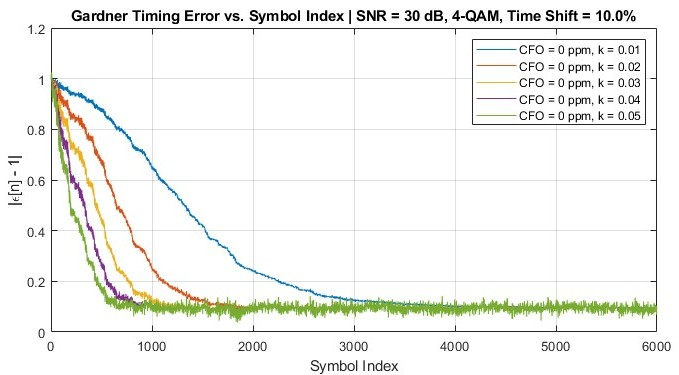
\includegraphics[scale=0.5]{Images/Gardner_k_list.jpg}
		\caption{Convergence of time shift error for different error weights k}
		\label{fig:gardner1}
	\end{figure}
	
	\begin{figure}[H]
		\centering
		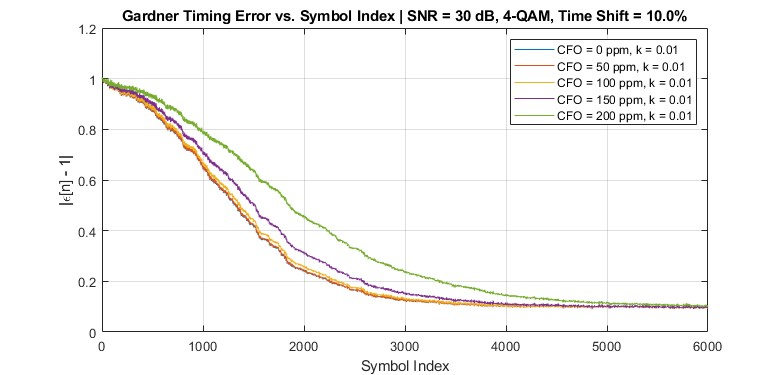
\includegraphics[scale=0.5]{Images/Gardner_CFO_robust.jpg}
		\caption{Robustness of the Gardner algorithm to the CFO}
		\label{fig:gardner2}
	\end{figure}
	
	
	
\end{document}
